% !TEX TS-program = pdflatex
% !TEX encoding = UTF-8 Unicode

% This file is a template using the "beamer" package to create slides for a talk or presentation
% - Talk at a conference/colloquium.
% - Talk length is about 20min.
% - Style is ornate.

% MODIFIED by Jonathan Kew, 2008-07-06
% The header comments and encoding in this file were modified for inclusion with TeXworks.
% The content is otherwise unchanged from the original distributed with the beamer package.

\documentclass{beamer}


% Copyright 2004 by Till Tantau <tantau@users.sourceforge.net>.
%
% In principle, this file can be redistributed and/or modified under
% the terms of the GNU Public License, version 2.
%
% However, this file is supposed to be a template to be modified
% for your own needs. For this reason, if you use this file as a
% template and not specifically distribute it as part of a another
% package/program, I grant the extra permission to freely copy and
% modify this file as you see fit and even to delete this copyright
% notice. 


\mode<presentation>
{
  \usetheme{Warsaw}
  % or ...

  \setbeamercovered{transparent}
  % or whatever (possibly just delete it)
}

\usepackage{graphics}

\usepackage[english]{babel}
% or whatever

\usepackage[utf8]{inputenc}
% or whatever

\usepackage{times}
\usepackage[T1]{fontenc}
% Or whatever. Note that the encoding and the font should match. If T1
% does not look nice, try deleting the line with the fontenc.
\newcommand*{\newblock}{}
\usepackage[round]{natbib}
\bibliographystyle{apalike}

\title[GAM Revisited] % (optional, use only with long paper titles)
{Putting the Geographical Analysis Machine on the Internet Revisited}

%\subtitle{Include Only If Paper Has a Subtitle}

\author[Turton, Turner] % (optional, use only with lots of authors)
{Ian~Turton\inst{1} \and Andrew Turner\inst{2}}
% - Give the names in the same order as the appear in the paper.
% - Use the \inst{?} command only if the authors have different
%   affiliation.

\institute[ ] % (optional, but mostly needed)
{
  \inst{1}%
Independent Researcher\\
 ijturton@gmail.com
  \and
  \inst{2}%
  Centre for Computational Geography\\
  University of Leeds\\
  A.G.D.Turner@leeds.ac.uk}
% - Use the \inst command only if there are several affiliations.
% - Keep it simple, no one is interested in your street address.

\date[ ] % (optional, should be abbreviation of conference name)
{GeoComputation 2011}
% - Either use conference name or its abbreviation.
% - Not really informative to the audience, more for people (including
%   yourself) who are reading the slides online


% If you have a file called "university-logo-filename.xxx", where xxx
% is a graphic format that can be processed by latex or pdflatex,
% resp., then you can add a logo as follows:

% \pgfdeclareimage[height=0.5cm]{university-logo}{university-logo-filename}
% \logo{\pgfuseimage{university-logo}}



% Delete this, if you do not want the table of contents to pop up at
% the beginning of each subsection:
\AtBeginSubsection[]
{
  \begin{frame}<beamer>{Outline}
    \tableofcontents[currentsection,currentsubsection]
  \end{frame}
}


% If you wish to uncover everything in a step-wise fashion, uncomment
% the following command: 

%\beamerdefaultoverlayspecification{<+->}


\begin{document}

\begin{frame}
  \titlepage
\end{frame}

\begin{frame}{Outline}
  \tableofcontents
  % You might wish to add the option [pausesections]
\end{frame}


\section{Introduction}
\begin{frame}[t]
\frametitle{Introduction}
\begin{itemize}
\item GAM - find clusters of cancer, first developed late 1980s
\item Gam/K on the Internet (late 1990s), attempt to bring tools to wider audience
\item Not as successful as we hoped :-(
\item Is the Internet and related web mapping technology ready for GAM now?
\end{itemize}
\end{frame}
\begin{frame}
\begin{columns}
\column{.5\textwidth}
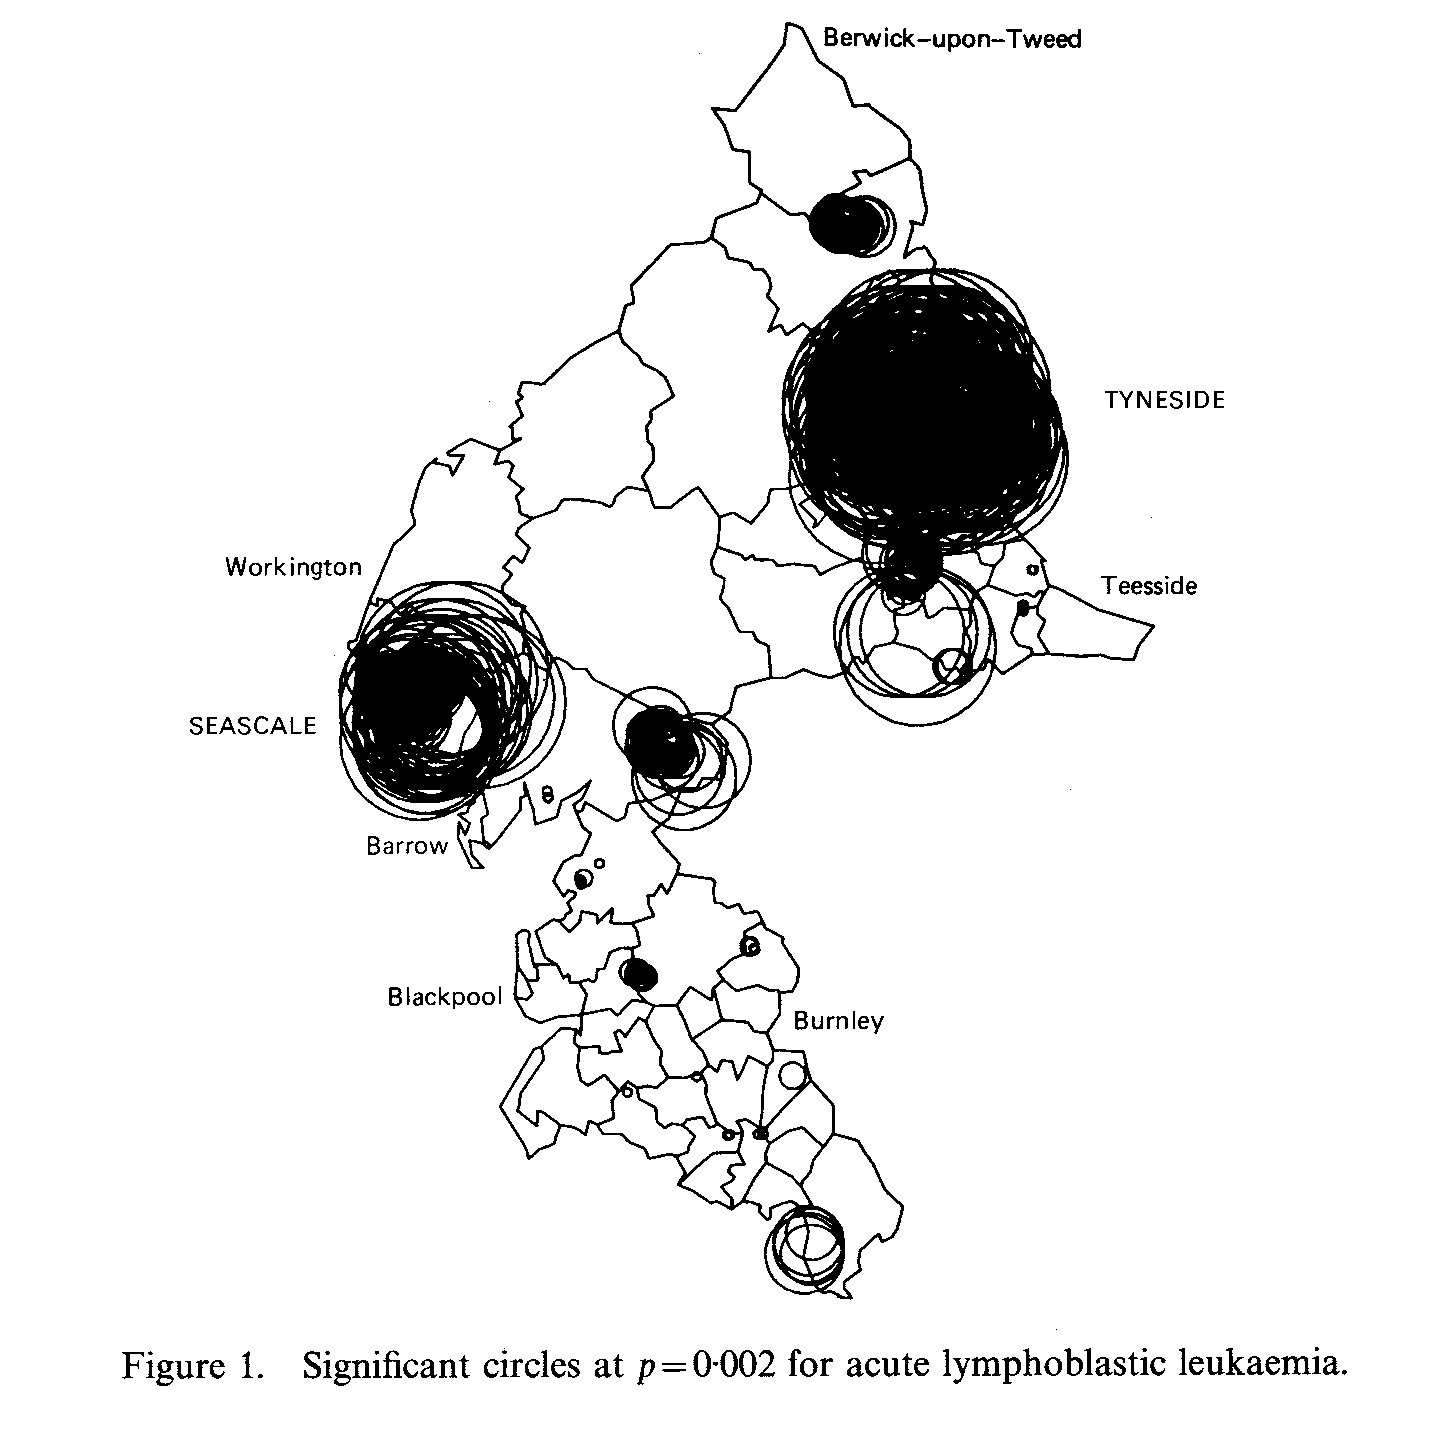
\includegraphics[height=6.0cm]{first_gam.png}
\column{.5\textwidth}
From \citet{citeulike:5207314}, note how early versions of GAM just drew circles.
\end{columns}
\end{frame}
\section{Motivation}
\begin{frame}[t]
\frametitle{Cancer Clusters}
\begin{itemize}
\item Earlier this year the Committee on Medical Aspects of Radiation in the Environment
(COMARE) released it's fourteenth report \href{http://www.comare.org.uk/press_releases/documents/COMARE14report.pdf}{\textit{
Further consideration of the incidence of childhood leukaemia around
nuclear power plants in Great Britain}} which reported that there was no evidence of childhood cancer clusters around British nuclear power plants.
\item Sadly hardly anyone believed them.
\end{itemize}
\end{frame}
\begin{frame}[t]
\frametitle{Motivation}

\begin{itemize}
\item Epidemiologists need powerful tools to help them find clusters of diseases in the large databases that they collect.
\item Current tools are hard to use, esoteric setup and formats to be mastered
\begin{itemize}
\item \citet{citeulike:6854836} state that "...training and software availability were cited as the primary barriers to the uptake of space-time disease surveillance..." and provide a general assessment that for the programs they tested - handling the data formatting was difficult and the interpretation of outputs was challenging.
\end{itemize}
\item So can we create a simple turn key tool set that allows them to run sophisticated analysis at the press of a button?
\end{itemize}
\end{frame}
\section{Implementation}
\begin{frame}[t]
\frametitle{Web Map Servers (WMS)}
\begin{itemize}
\item A simple standard that allows web browsers to download pictures of maps
\item Ideal if the end user has little or no GIS experience (or doesn’t want to pay for ArcMap). 
\item Can be served on top of Google maps for easy base map provision
\item \textbf{We will use WMS to provide easy access to the results of our analysis}
\end{itemize}
\end{frame}
\begin{frame}[t]
\frametitle{Web Feature Server (WFS)}
\begin{itemize}
\item Serve up actual geographic data 
\item useful for sharing vector data from a central repository to many users
\item \textbf{We will use WFS to provide the inputs to our analysis}
\end{itemize}
\end{frame}
\begin{frame}[t]
\frametitle{Web Processing Standard (WPS)}
\begin{itemize}

\item A newer OGC standard \citep{OGC2007} that provides a defined protocol for executing remote processes on geographic data.
\item Can take inputs from WFS servers or local files
\item Advanced users can define a sub WPS process to produce the population at risk using a model.
\item returns results as downloadable files or WMS results
\end{itemize}
\end{frame}


\begin{frame}[t]
\frametitle{GeoTools}
\begin{itemize}
\item GeoTools is an open source Java library for geospatial operations \citep{Hall2008}
\item GeoTools provides an abstracted datastore model, simple features and a variety of OGC standards (Filtering, Styling etc).
\item Code and documentation are available at \url{http://geotools.org}
\end{itemize}
\end{frame}

\begin{frame}[t]
\frametitle{GeoServer}
\begin{itemize}
\item High quality WMS/WFS/WCS/WPS
\item used to serve up maps by many European NMA (GB,FR,NL...)
\item Based on the GeoTools code base so integration is easy
\item Download it and try for your self from \url{http://geoserver.org}
\end{itemize}
\end{frame}

\begin{frame}[t]
\frametitle{Clustering Code}
\begin{itemize}
\item First developed under ESRC funding in FORTRAN
\item Rewritten in Java under EU Spin! grant
\item Now completely rewritten to use GeoTools and WPS processing tools
\item Go to \url{http://code.google.com/p/spatial-cluster-detection/} to try out the code or join us in development, 
\end{itemize}
\end{frame}

\section{Results}
\begin{frame}[t]
\frametitle{}
\end{frame}

\section{Conclusions}
\begin{frame}[t]
\frametitle{Conclusions}
\begin{itemize}
\item It works
\item It needs more work 
\item Would you like to help? Go to \href{http://code.google.com/p/spatial-cluster-detection/}{http://code.google.com/p/spatial-cluster-detection/}
\end{itemize}
\end{frame}


\begin{frame}[allowframebreaks]
  \frametitle<presentation>{For Further Reading}
    
\bibliography{clustering,ogc}
\end{frame}

\end{document}


